\section{Поиск архитектуры глубокого обучения.}

В глубоком обучении по большей части используются градиентные
методы и численное дифференцирование, поэтому и функция
предсказания и функция ошибки должны быть дифференцируемы.

Архитектура задается ациклиеским графом, в каждой вершине мы
умеем вычислять производную по входу и параметрам. Можем юзать
бэкпроп.

Функции ошибки для регрессии обычно дифференцируемы. Классификацию
мы сводим к мягкой классификации.

Основной гиперпараметр - архитектура сети. (аналогичен по сложности
конфигурации гиперпараметров для традиционного алгоритма) Также
гиперпараметром может быть функция ошибок. Параметры градиентного
спуска также можно считать гиперпараметрами.

Фиксированное число слоев:
\begin{itemize}
    \item Полносвязные архитектуры (линейная конфигурация)
    \item Сверточные архитектуры (больше параметров)
    \item Графы (опираются на базовую функцию, архитектура
    которой может настраиваться)
\end{itemize}

Нефиксированное:
\begin{itemize}
    \item Пространство поиска усложняется
    \item Эвол. алг. требуют операторов для объектов переменной длины
    \item Последовательность переменной длины можно закодировать деревом
    \item Суррогатная функция в БО должна уметь обрабатывать последовательности
\end{itemize}

\subsubsection*{Произвольные ациклические графы}

Для эвол. алг:
\begin{itemize}
    \item Генерация: создается случайная вершина и соединяется с
    предыдущими
    \item Мутация: добавление или удаление вершин с присоединением ребер
    \item Кроссовер: склеивание частей графов
\end{itemize}

Для БО суррогатная функция должна уметь обрабатывать графы.

% \begin{figure}[H]
% 	\centering
% 	\begin{minipage}[b]{0.4\textwidth}
% 		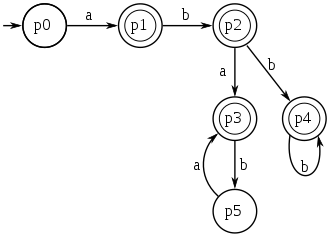
\includegraphics[width=\textwidth]{images/dfa.png}
% 		\caption{Пример графа переходов детерминированного КА.}
% 	\end{minipage}
% 	\hfill
% 	\begin{minipage}[b]{0.4\textwidth}
% 		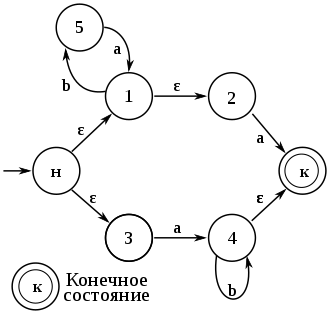
\includegraphics[width=\textwidth]{images/ndfa.png}
% 		\caption{Пример графа переходов недетерминированного КА с самопроизвольными переходами.}
% 	\end{minipage}
% \end{figure}